\documentclass[a4paper]{article}
\usepackage[utf8]{inputenc}
\usepackage[spanish, es-tabla, es-noshorthands]{babel}
\usepackage[table,xcdraw]{xcolor}
\usepackage[a4paper, footnotesep = 1cm, width=20cm, top=2.5cm, height=25cm, textwidth=18cm, textheight=25cm]{geometry}
%\geometry{showframe}

\usepackage{tikz}
\usepackage{amsmath}
\usepackage{amsfonts}
\usepackage{amssymb}
\usepackage{float}
\usepackage{graphicx}
\usepackage{caption}
\usepackage{subcaption}
\usepackage{multicol}
\usepackage{multirow}
\setlength{\doublerulesep}{\arrayrulewidth}
\usepackage{booktabs}
\usepackage{mathrsfs,amsmath}
\usepackage{hyperref}
\hypersetup{
    colorlinks=true,
    linkcolor=blue,
    filecolor=magenta,      
    urlcolor=blue,
    citecolor=blue,    
}

\newcommand{\quotes}[1]{``#1''}
\usepackage{array}
\newcolumntype{C}[1]{>{\centering\let\newline\\\arraybackslash\hspace{0pt}}m{#1}}
\usepackage[american]{circuitikz}
\usetikzlibrary{calc}
\usepackage{fancyhdr}
\usepackage{units} 

\graphicspath{./Imagenes}

\pagestyle{fancy}
\fancyhf{}
\lhead{22.05 ASSD}
\rhead{Mechoulam, Lambertucci, Rodriguez, Londero}
\rfoot{Página \thepage}

\begin{document}
\subsection{FFT}
Se implementó la FFT utilizando el algoritmo de Cooley-Tukey de manera recursiva.
Se probó con diversas entradas reales aleatorias, de tamaño 4096, con una media temporal de 40$\mu$s.
\subsection{Programa Principal}
La GUI implementada es la siguiente:
\begin{figure}[H]
	\centering
	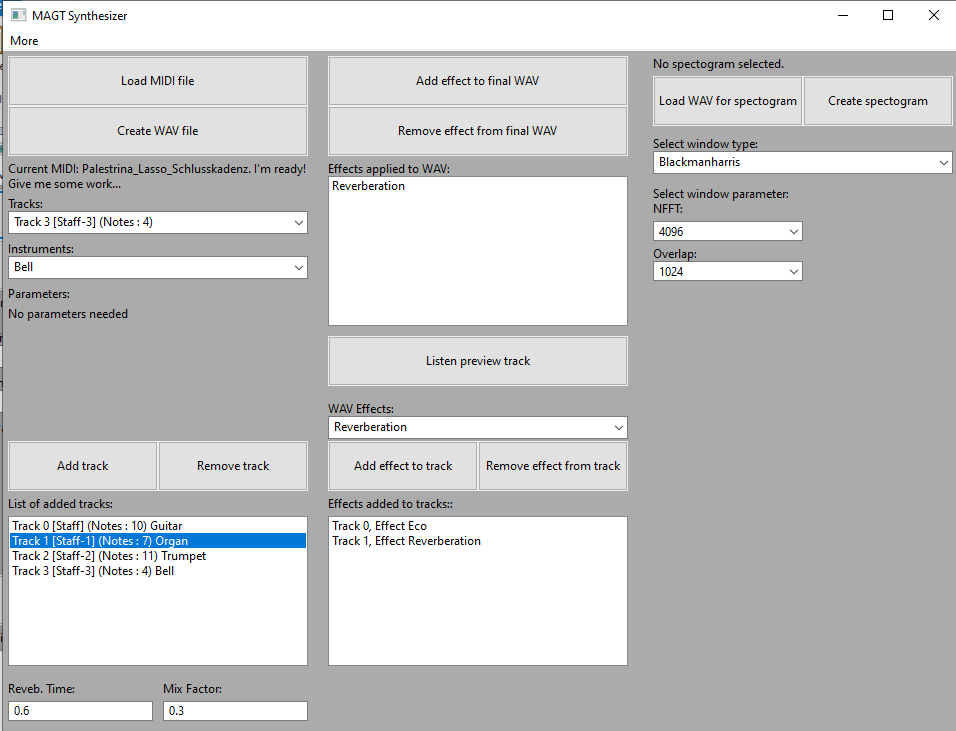
\includegraphics[width=0.8\textwidth]{ImagenesEjercicio8/GUI.PNG}
\caption{GUI Implementada.}
	\label{fig:gui}
\end{figure}
Permite agregar midis de cualquier duración, sintetizar cada track con el instrumento deseado, al igual que escuchar un preview del mismo, funcionalidad de pantalla completa, una sección de ayuda al usuari; Ademas permite la mezcla tracks, agregar efectos tanto a los tracks como al proyecto entero. Realizar espectrogramas de los wavs generados, pudiendo elegir el tipo de ventana, la cantidad de puntos de la FFT y el overlap. Ademas permite manejar los parametros de algunos instrumentos y efectos.\\
El front-end del programa se implemento en WxWidgets. El programa fue desarrollado en C++. \\

\end{document}